\markboth{CAPITOLO 4. ESERCIZI A.A. 2017-18}{CAPITOLO 4. ESERCIZI A.A. 2017-18}
\begin{flushleft}
\textbf{Esercizio 4.1} \textit{Scrivere una function Matlab che implementi il calcolo del polinomio interpolante di grado \textit{n} in forma di Lagrange. \\La forma della function deve essere del tipo: \lstinline[language=Matlab]{Capitolo4/y = lagrange( xi, fi, x )}}\\
\textbf{Soluzione: } \lstinputlisting[language=Matlab]{Capitolo4/es4_1.m}
\bigskip
\textbf{Esercizio 4.2} \textit{Scrivere una function Matlab che implementi il calcolo del polinomio interpolante di grado \textit{n} in forma di Newton. \\La forma della function deve essere del tipo: \lstinline[language=Matlab]{Capitolo4/y = newton( xi, fi, x )}}\\
\textbf{Soluzione: } \lstinputlisting[language=Matlab]{Capitolo4/es4_2.m}
\bigskip
\textbf{Esercizio 4.3} \textit{Scrivere una function Matlab che implementi il calcolo del polinomio interpolante di Hermite. \\La forma della function deve essere del tipo: \lstinline[language=Matlab]{Capitolo4/y = hermite( xi, fi, f1i, x )}}\\
\textbf{Soluzione: }  \lstinputlisting[language=Matlab]{Capitolo4/es4_3.m}
\newpage
\textbf{Esercizio 4.4} \textit{Utilizzare le functions degli esercizi precedenti per disegnare l'approssimazione della funzione \(\sin(x)\) nell'intervallo \([0, 2\pi]\), utilizzando le ascisse di interpolazione \(x_i=i\pi\), \(i= 0,1,2\).}\\
\textbf{Soluzione: }
\begin{center}
	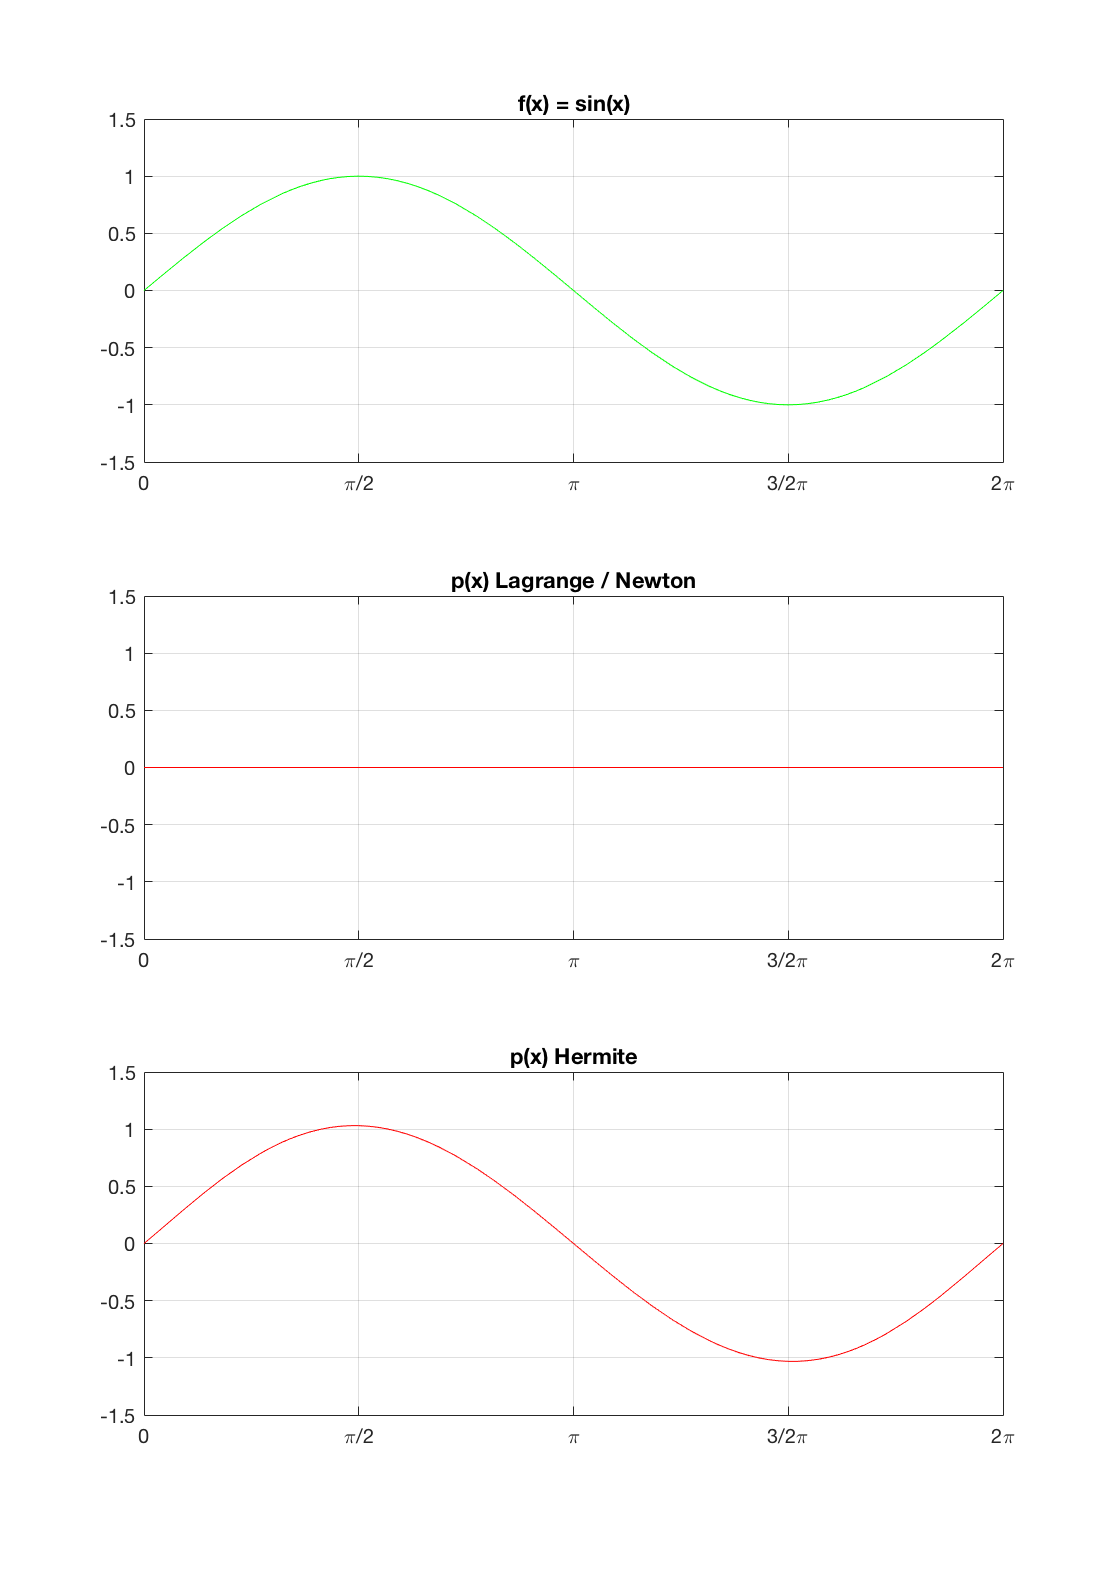
\includegraphics[scale=0.31]{Capitolo4/es4_4.png}
\end{center}
Possiamo notare come il polinomio di Lagrange e Newton genera una retta $y=0$ essendo $f_{i} = 0$ in tutte le ascisse.
\lstinputlisting[language=Matlab]{Capitolo4/es4_4.m}
\bigskip
\textbf{Esercizio 4.5} \textit{Scrivere una function Matlab che implementi la spline cubica interpolante (naturale o \textit{not-a-knot}, come specificato in ingresso) delle coppie di dati assegnate. La forma della funcion deve essere del tipo: \lstinline[language=Matlab]{Capitolo4/y = spline3(xi, fi, x, tipo)}}\\
\textbf{Soluzione: } Il seguente codice Matlab implementa la function richiesta. Per rendere il codice pi� leggibile sono state craete varie sottofunzioni.\\ Il codice � stato testato con un banale esempio:
\lstinputlisting[language=Matlab]{Capitolo4/es4_5.m}
\bigskip
\textbf{Esercizio 4.6} \textit{Scrivere una function Matlab che implementi il calcolo delle ascisse di Chebyshev per il polinomio interpolante di grado \textit{n}, su un generico intervallo \([a, b]\). \\La function deve essere del tipo: \lstinline[language=Matlab]{Capitolo4/ xi = ceby( n, a, b )}}\\
\textbf{Soluzione: }
\lstinputlisting[language=Matlab]{Capitolo4/es4_6.m}
\newpage
\textbf{Esercizio 4.7} \textit{Utilizzare le function degli Esercizi 4.1 e 4.6 per graficare l'approssimazione della funzione di Runge sull'intervallo \([-6, 6]\), per \(n = 2, 4, 6, \ldots, 40\). Stimare numericamente l'errore commesso in funzione del grado \textit{n} del polinomio interpolante.}\\
\textbf{Soluzione: } Di seguito i grafici che mostrano i polinomi interpolanti di grado \textit{n} calcolati utilizzando come punti di interpolazione quelli corrispondenti alle \textit{n} ascisse di Chebyshev, sovrapposti al grafico della funzione di Runge: \(f(x) = \frac{1}{1+x^2}\). \\
\begin{tabular}{c c}
\(n=2\) & \(n=4\) \\
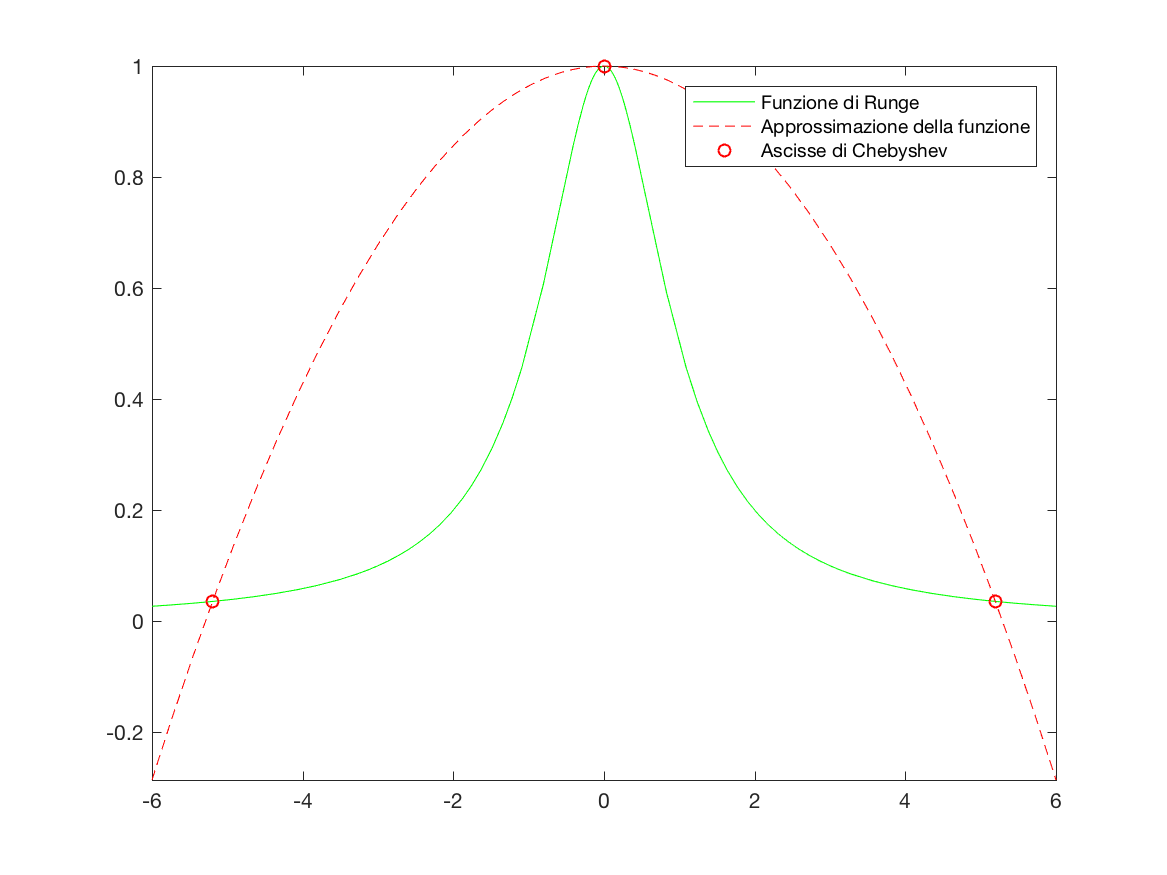
\includegraphics[scale=0.333]{Capitolo4/graficiEs7/es4_7_img2.png} &  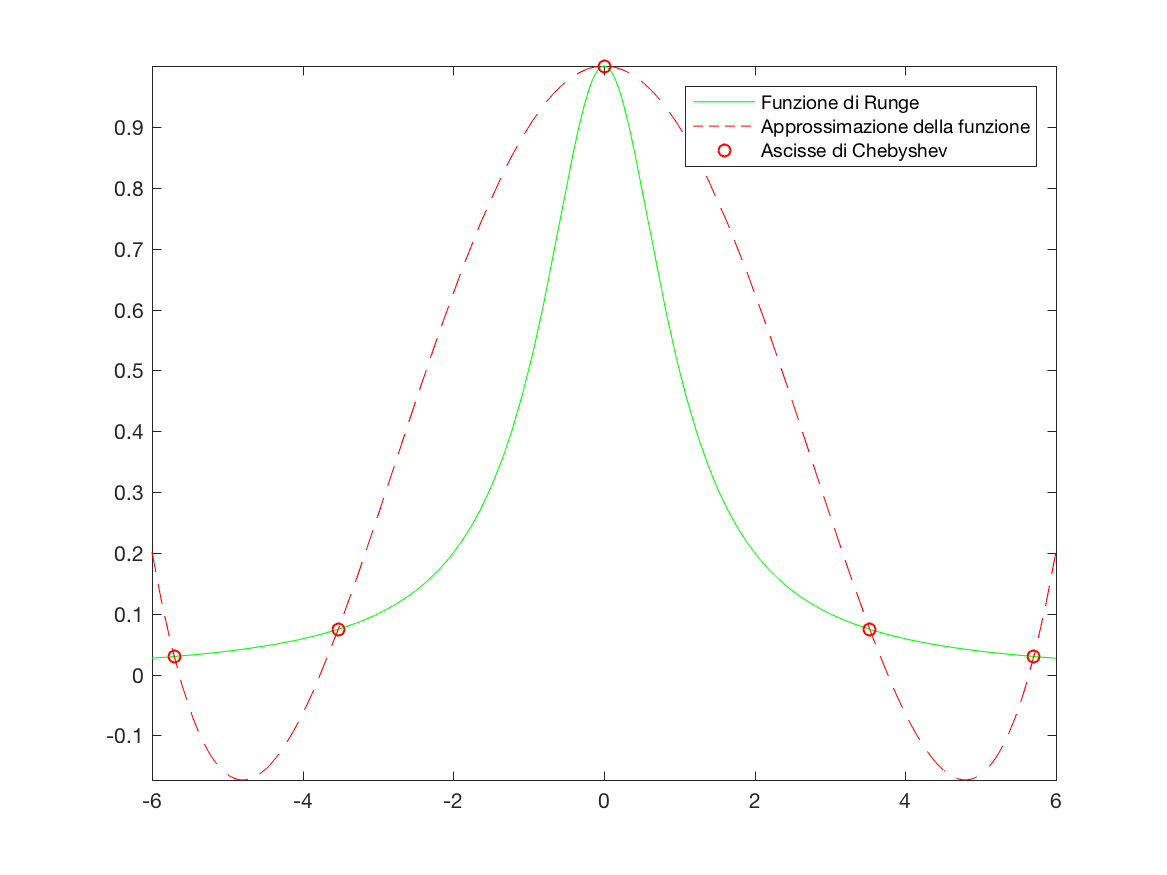
\includegraphics[scale=0.333]{Capitolo4/graficiEs7/es4_7_img4.png} \\
\(n=6\)& \(n=8\) \\
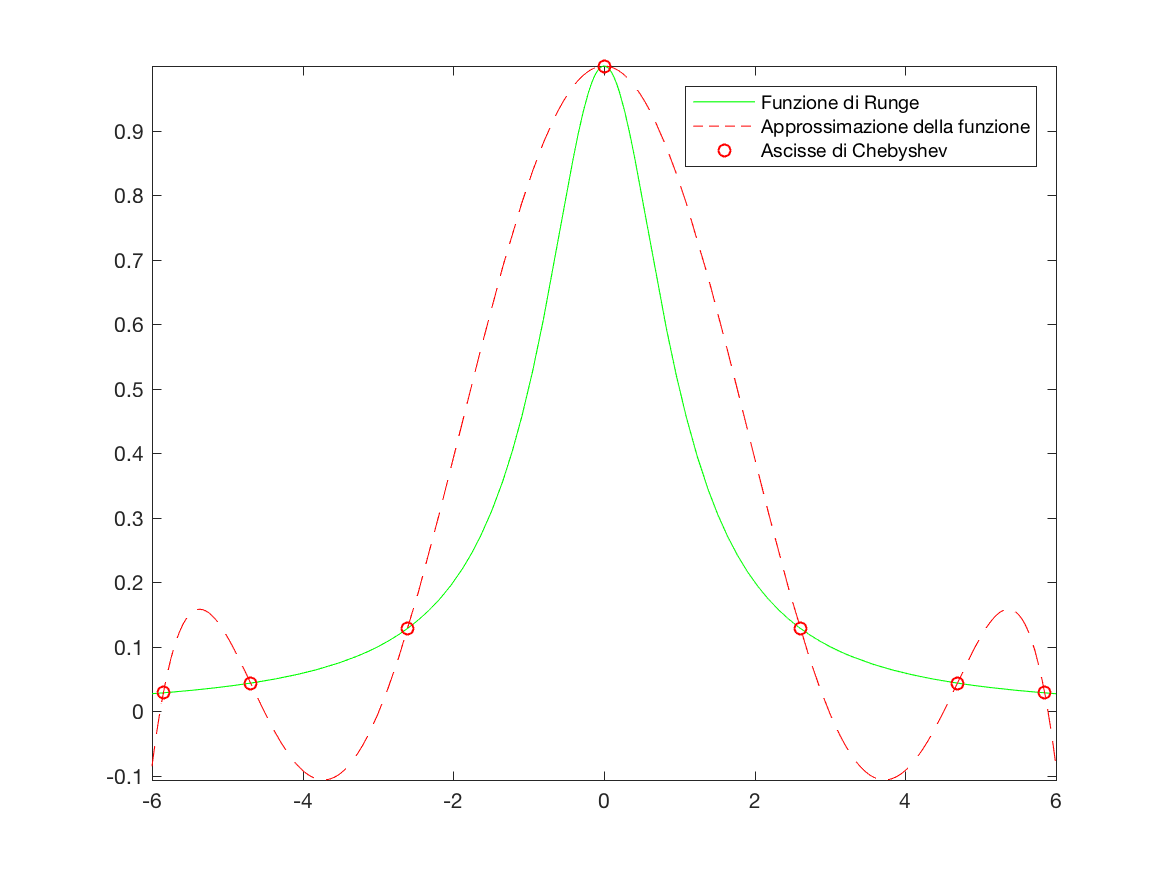
\includegraphics[scale=0.333]{Capitolo4/graficiEs7/es4_7_img6.png} &  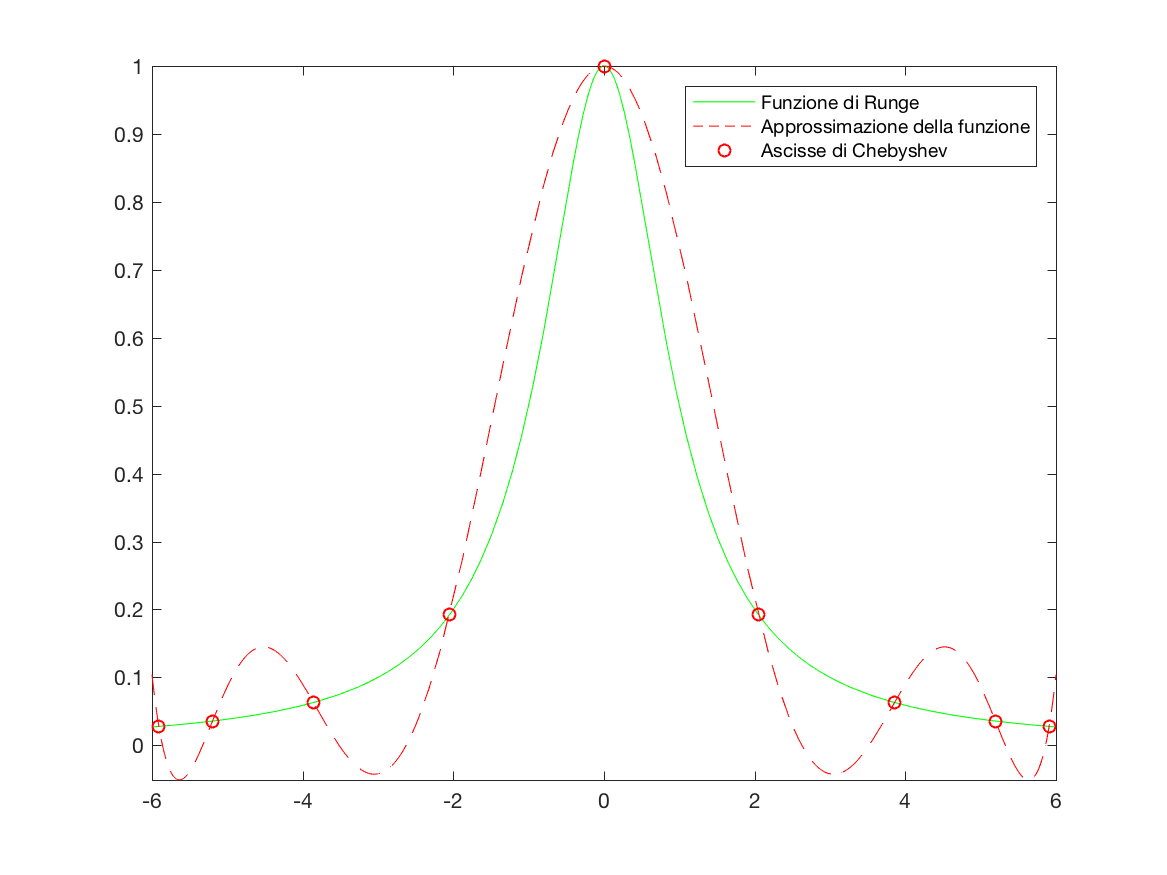
\includegraphics[scale=0.333]{Capitolo4/graficiEs7/es4_7_img8.png} \\
\(n=10\) &  \(n=12\) \\
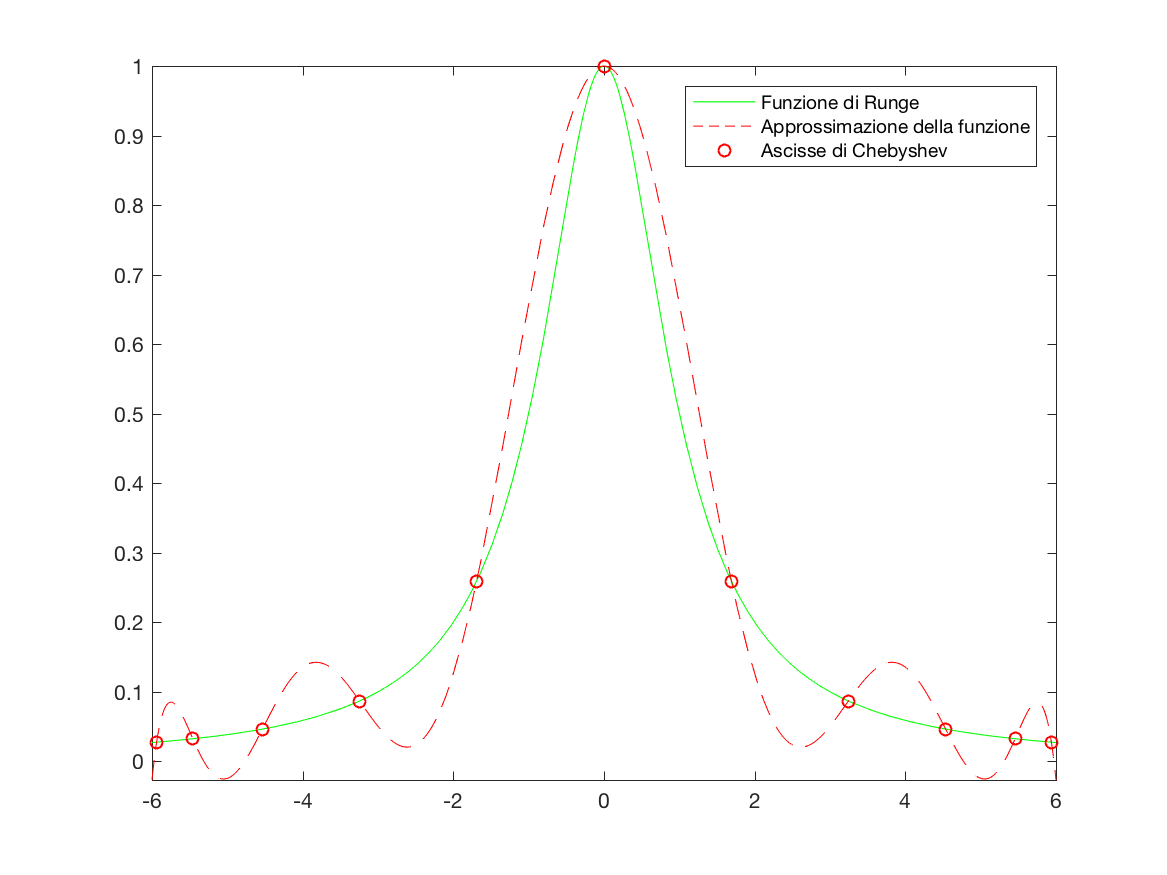
\includegraphics[scale=0.333]{Capitolo4/graficiEs7/es4_7_img10.png} &  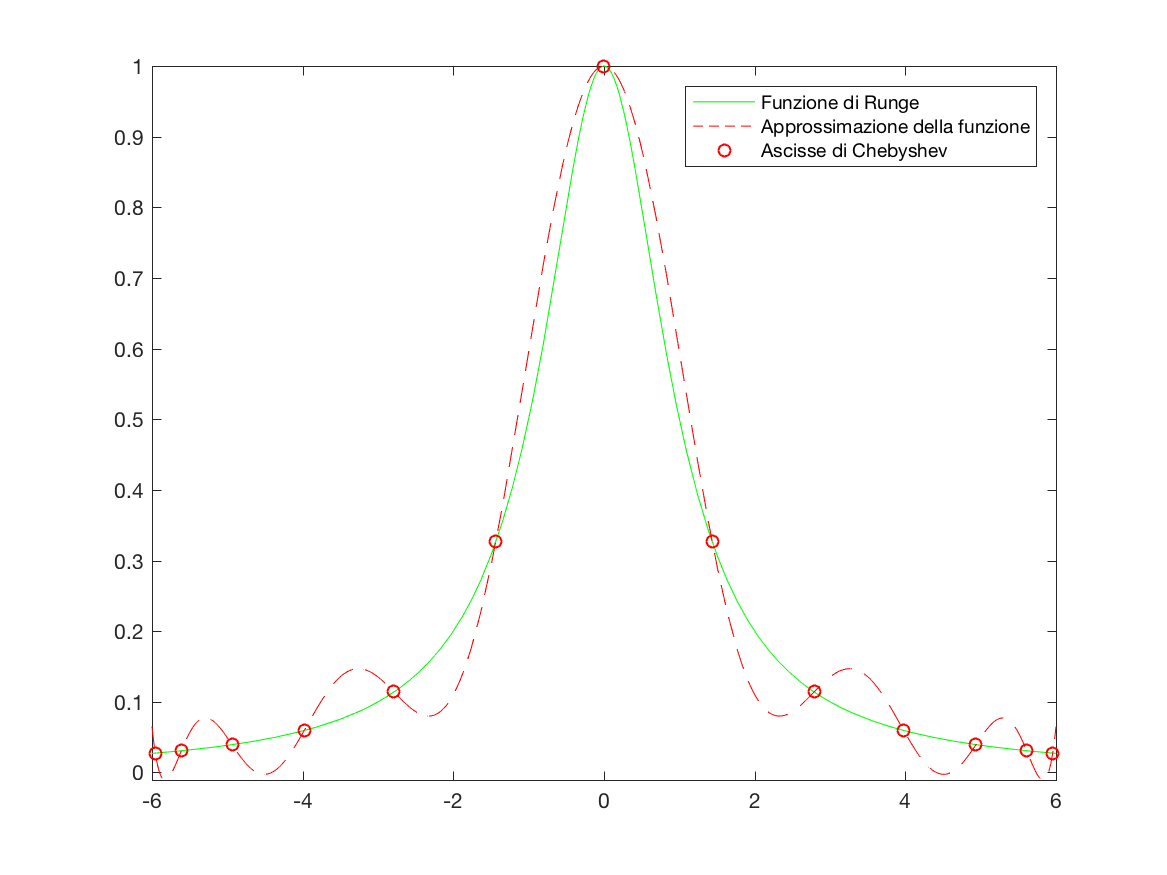
\includegraphics[scale=0.333]{Capitolo4/graficiEs7/es4_7_img12.png} \\
\end{tabular} \\
\noindent\begin{tabular}{c c}
\(n=16\) & \(n=22\) \\
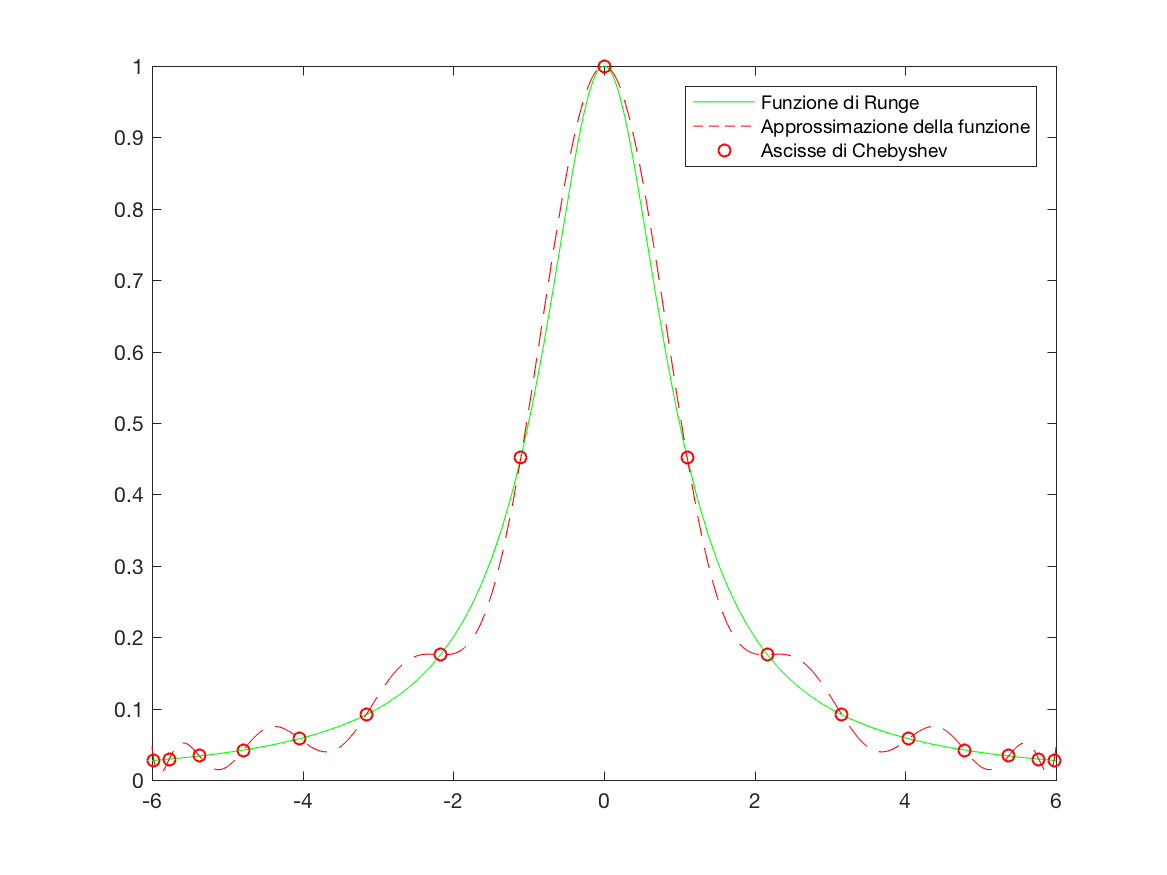
\includegraphics[scale=0.333]{Capitolo4/graficiEs7/es4_7_img16.png} &  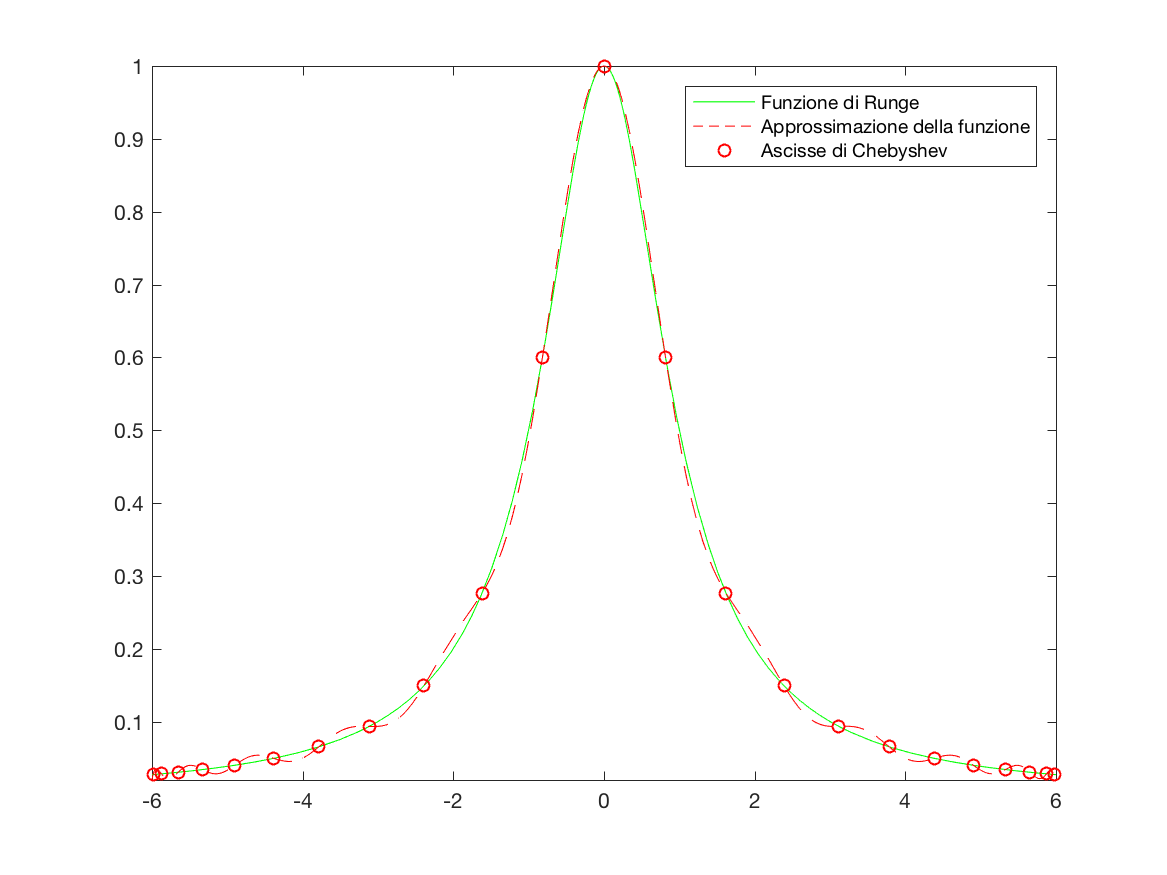
\includegraphics[scale=0.333]{Capitolo4/graficiEs7/es4_7_img22.png} \\
\(n=28\)& \(n=30\) \\
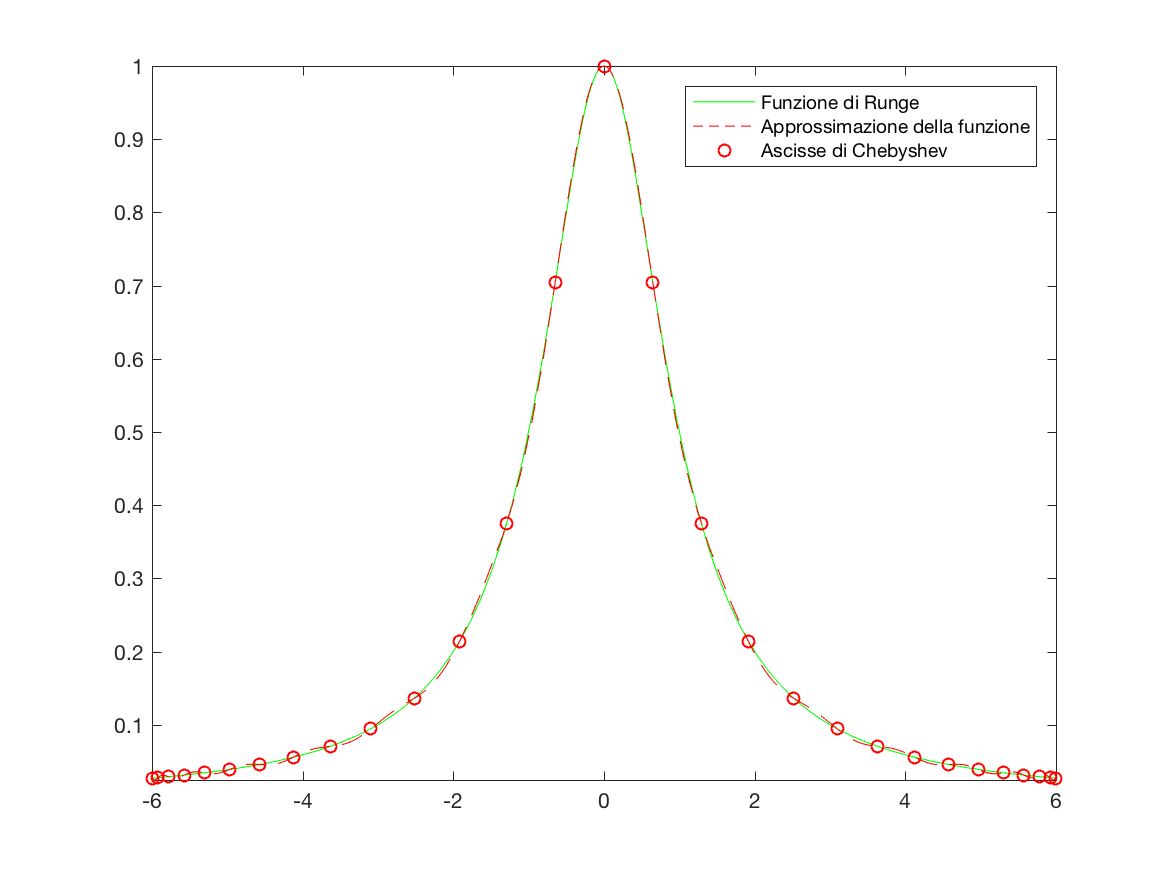
\includegraphics[scale=0.333]{Capitolo4/graficiEs7/es4_7_img28.png} &  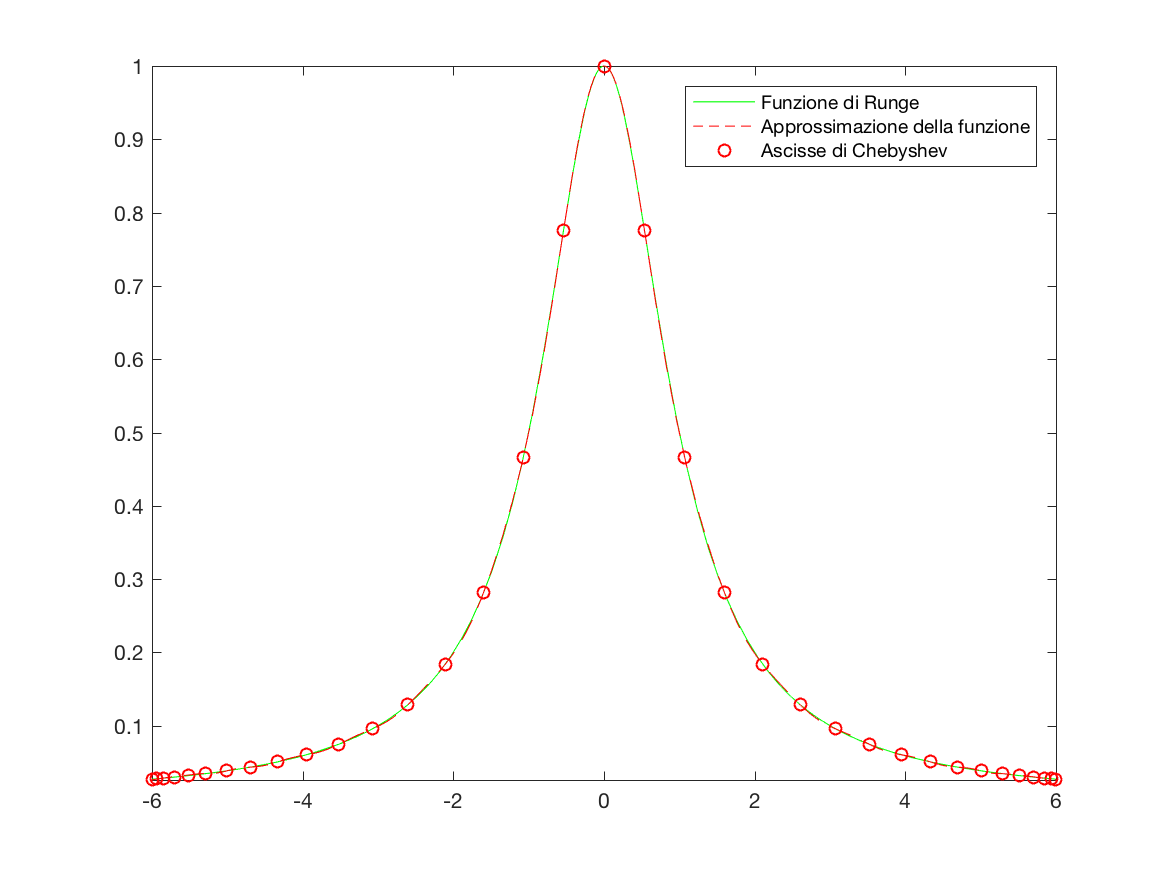
\includegraphics[scale=0.333]{Capitolo4/graficiEs7/es4_7_img34.png} \\
\(n=40\) &  \\
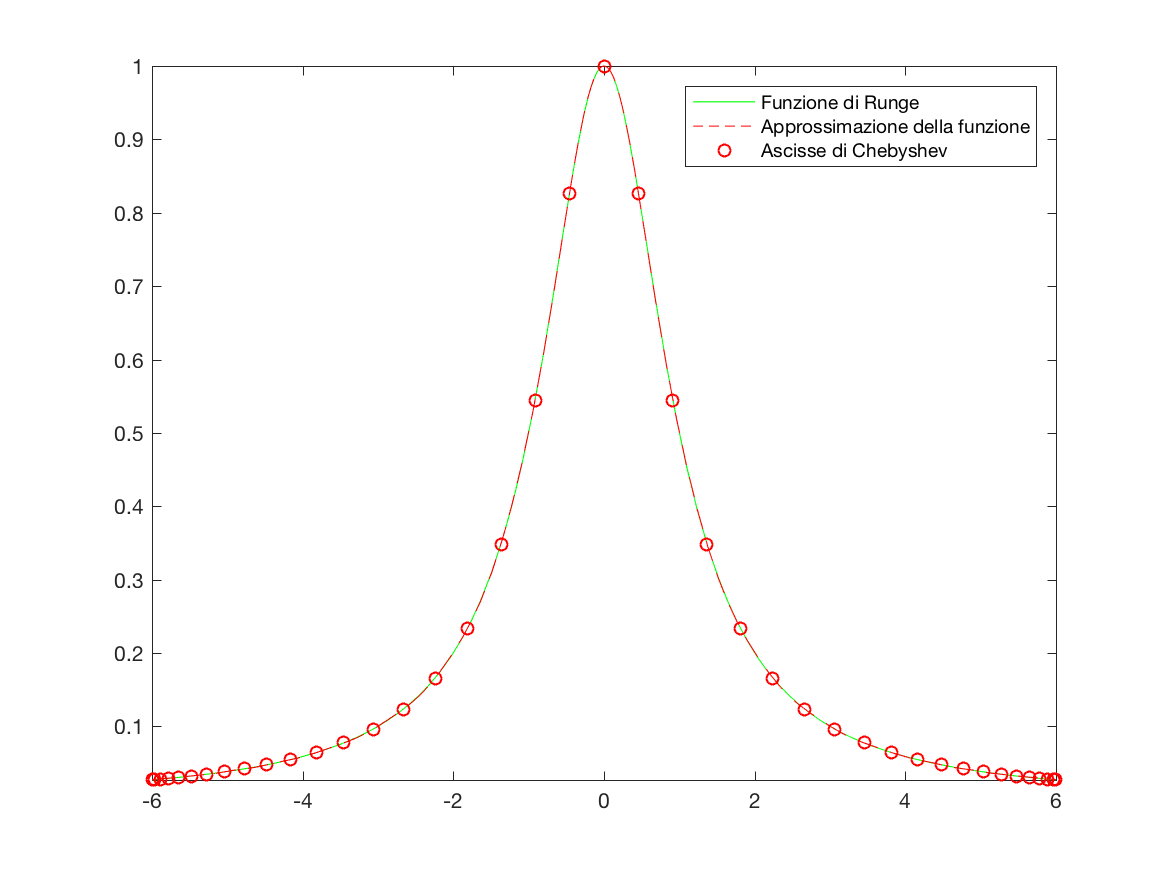
\includegraphics[scale=0.333]{Capitolo4/graficiEs7/es4_7_img40.png} &   \\
\end{tabular} \\
L'errore � stato calcolato seguendo la seguente formula:
$$
||e|| \approx ||f(x) - p_n(x)||_{\inf}
$$
Dove $f$ � intesa come la funzione di Runge e $p$ il suo polinomio interpolante.
\newpage
L'errore stimato � visibile nella seguente tabella:
\begin{center}
	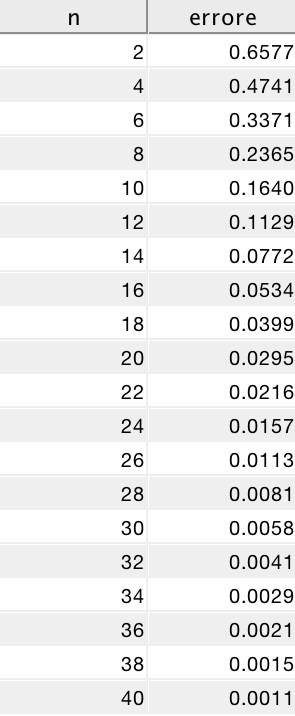
\includegraphics[scale=0.4]{Capitolo4/es4_7_tabErrore.png}
\end{center}
Notiamo che, utilizzando le ascisse di Chebyshev, aumentando il numero di punti otteniamo un'approssiamazione sempre pi� vicina alla funzione di Runge. Infatti l'errore diminuisce all'aumentare di n tendendo a 0 quando n tende all'infinito.

\bigskip
\textbf{Esercizio 4.8} \textit{Relativamente al precedente esercizio, stimare numericamente la crescita della costante di Lebesgue.}\\
\textbf{Soluzione: } La stima della costante di Lebesgue mediante le ascisse di Chebyshev � data dalla seguente formula:
\[
\Lambda_n \approx \frac{2}{\pi}\log n
\]
Ci si aspetta quindi che abbia una crescita logaritmica al crescere di \(n\).
\newpage
La tebella seguente  mette in evidenza tale comportamento:
\begin{center}
	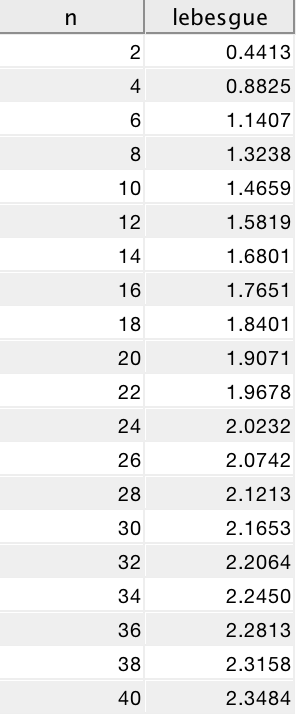
\includegraphics[scale=0.4]{Capitolo4/es4_8_tabella.png}
\end{center}

\bigskip
\textbf{Esercizio 4.9} \textit{Utilizzare la function ell'Esercizio 4.1 per approssimare la funzione di Runge sull'intervallo \([-6, 6]\), su una partizione uniforme di \(n+1\) ascisse per \(n = 2, 4, 6, \ldots, 40\). Stimare le corrispondenti costanti di Lebesgue.}\\
\textbf{Soluzione: }
\begin{tabular}{cc}
\(n=2\) & \(n=4\) \\
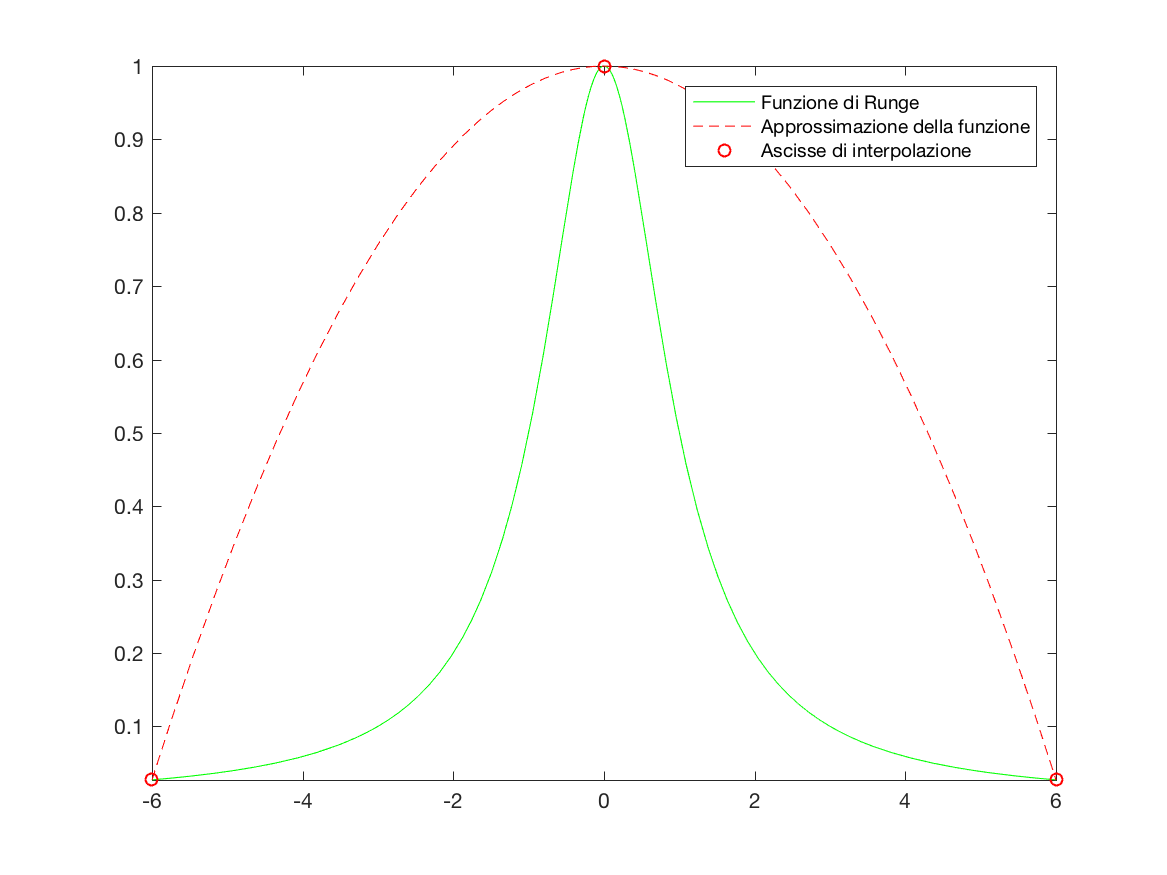
\includegraphics[scale=0.333]{Capitolo4/graficiEs9/es4_9_img2.png} &  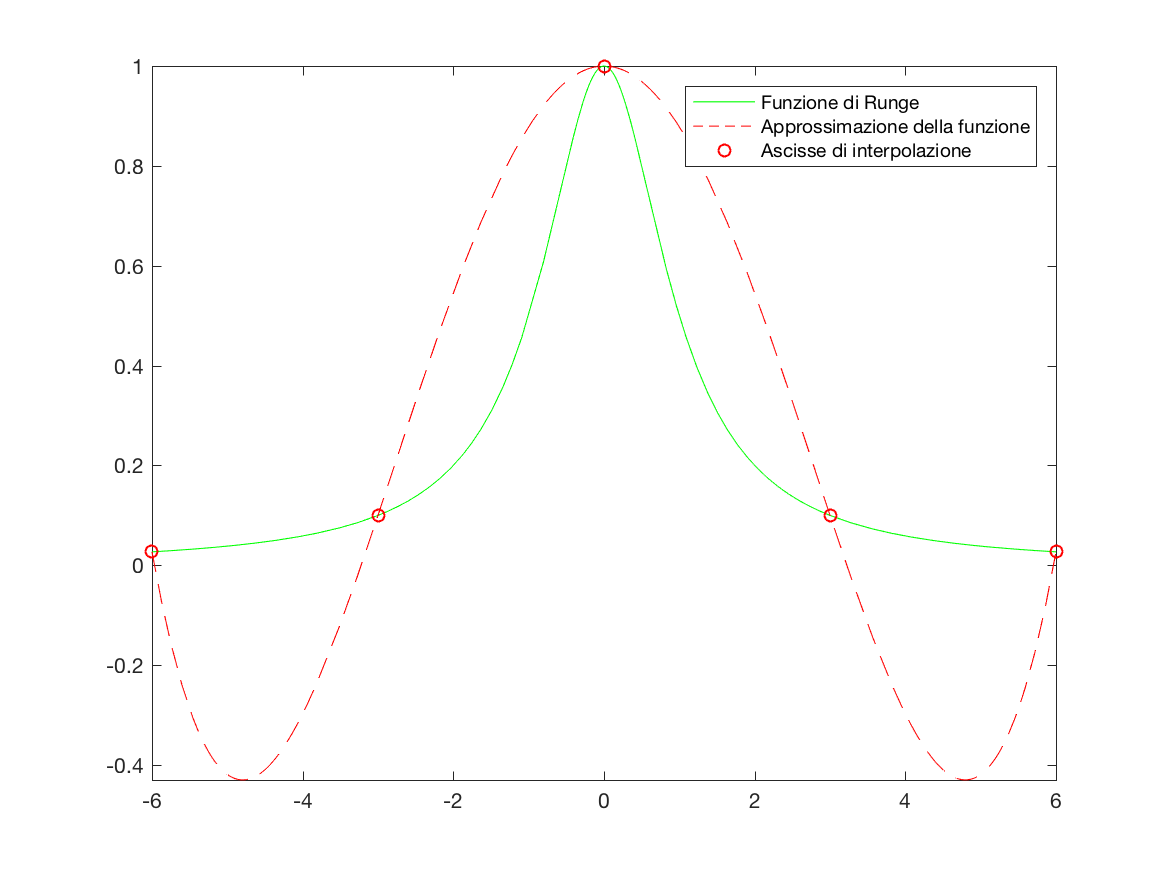
\includegraphics[scale=0.333]{Capitolo4/graficiEs9/es4_9_img4.png} \\
\end{tabular} \\
\begin{tabular}{cc}
\(n=6\) & \(n=8\) \\
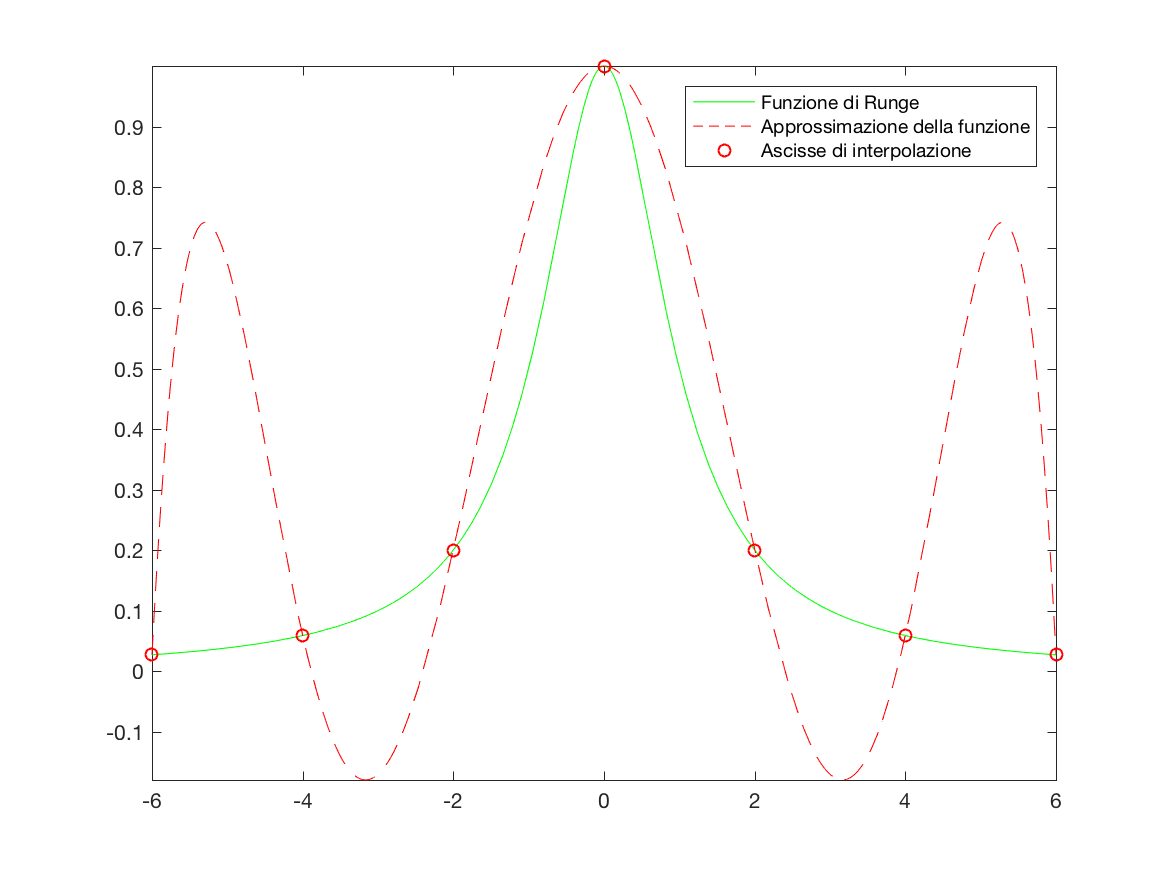
\includegraphics[scale=0.333]{Capitolo4/graficiEs9/es4_9_img6.png} &  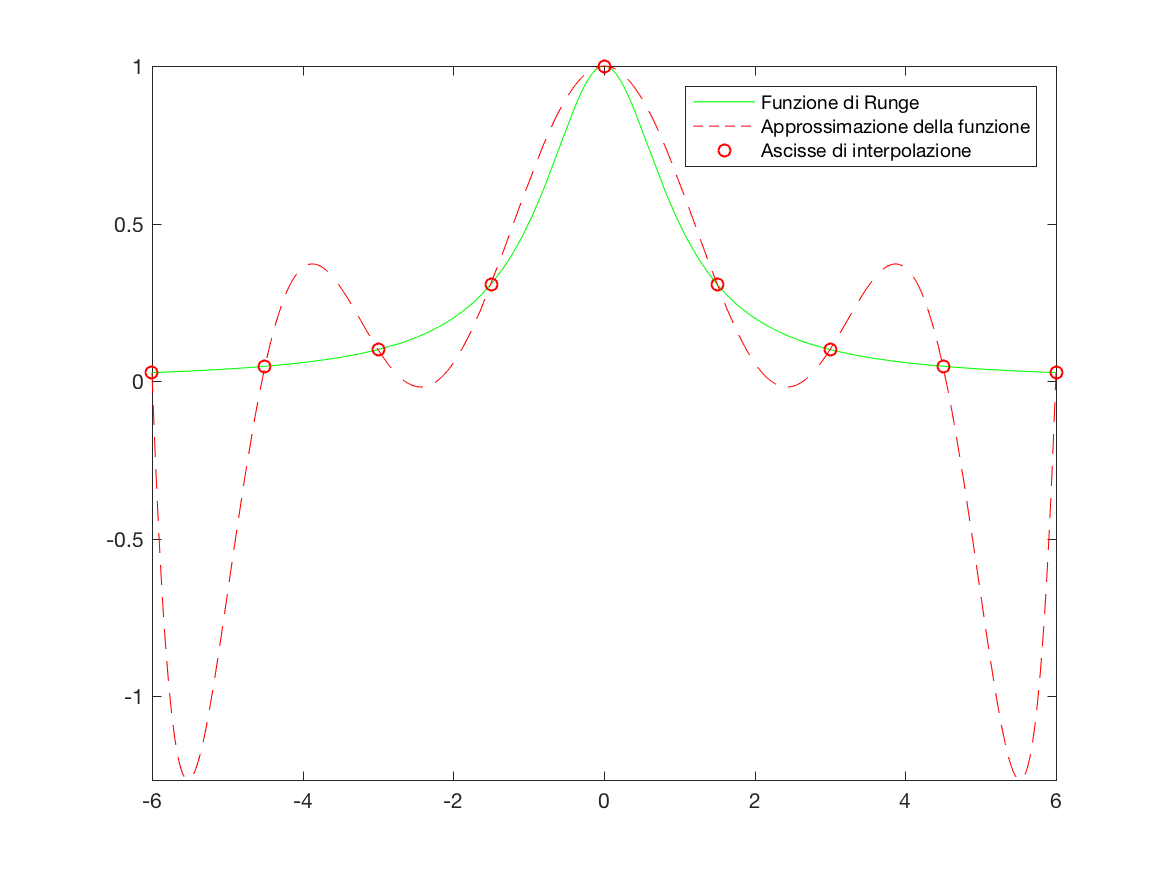
\includegraphics[scale=0.333]{Capitolo4/graficiEs9/es4_9_img8.png} \\
\(n=10\) & \(n=12\) \\
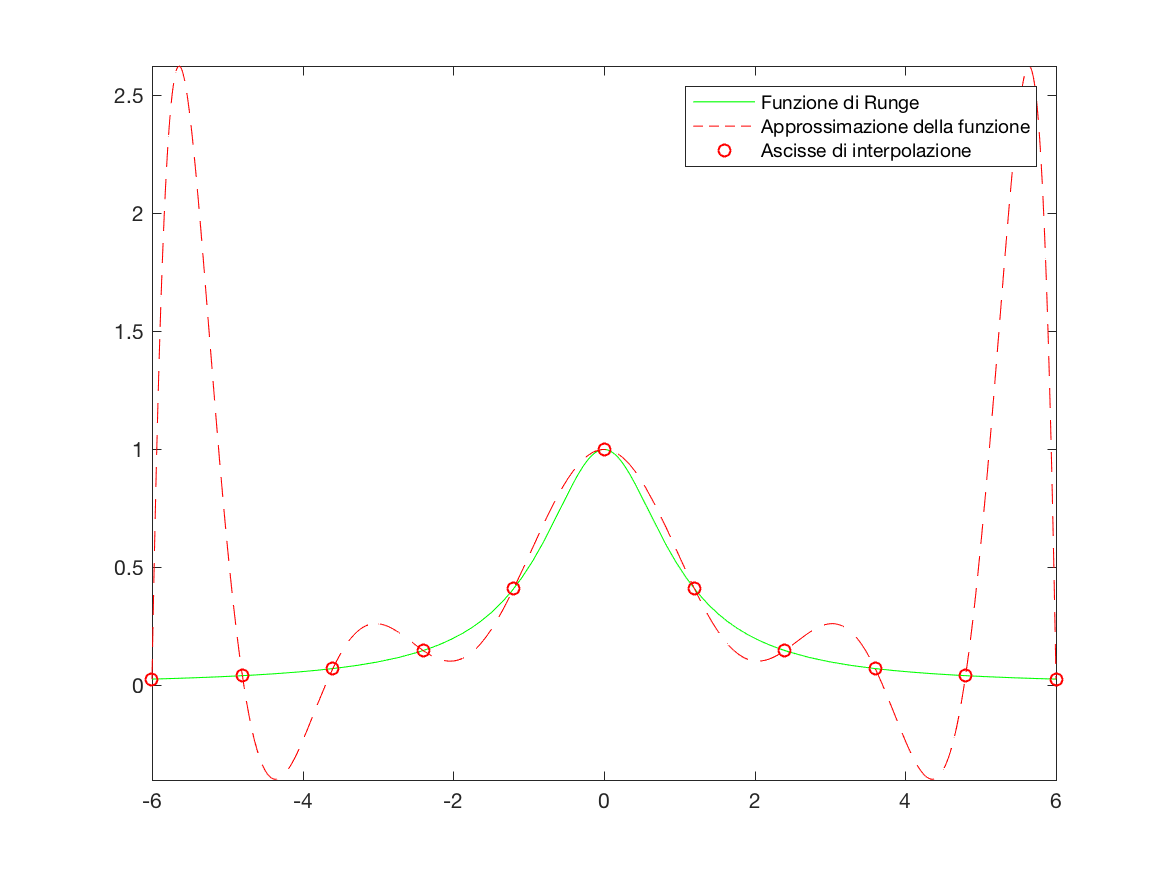
\includegraphics[scale=0.333]{Capitolo4/graficiEs9/es4_9_img10.png} &  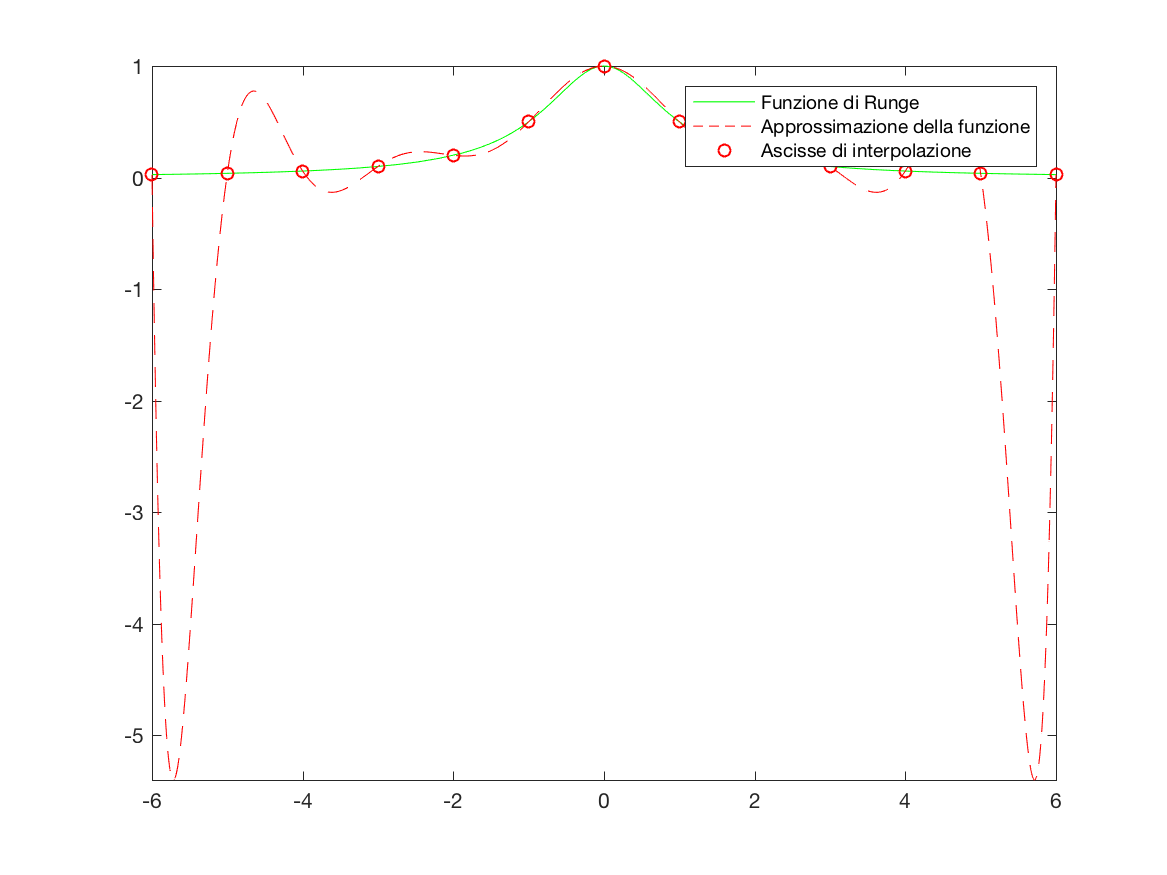
\includegraphics[scale=0.333]{Capitolo4/graficiEs9/es4_9_img12.png} \\
\(n=16\) & \(n=22\) \\
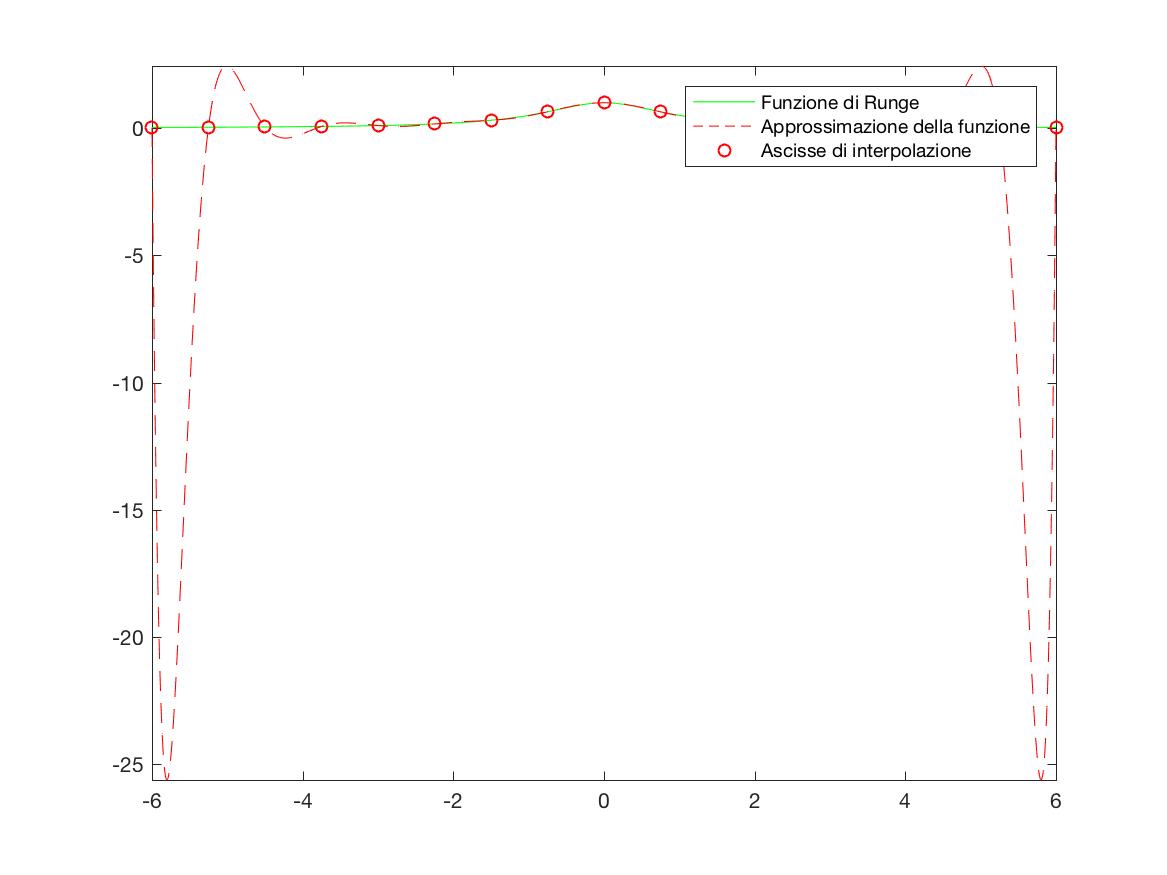
\includegraphics[scale=0.333]{Capitolo4/graficiEs9/es4_9_img16.png} &  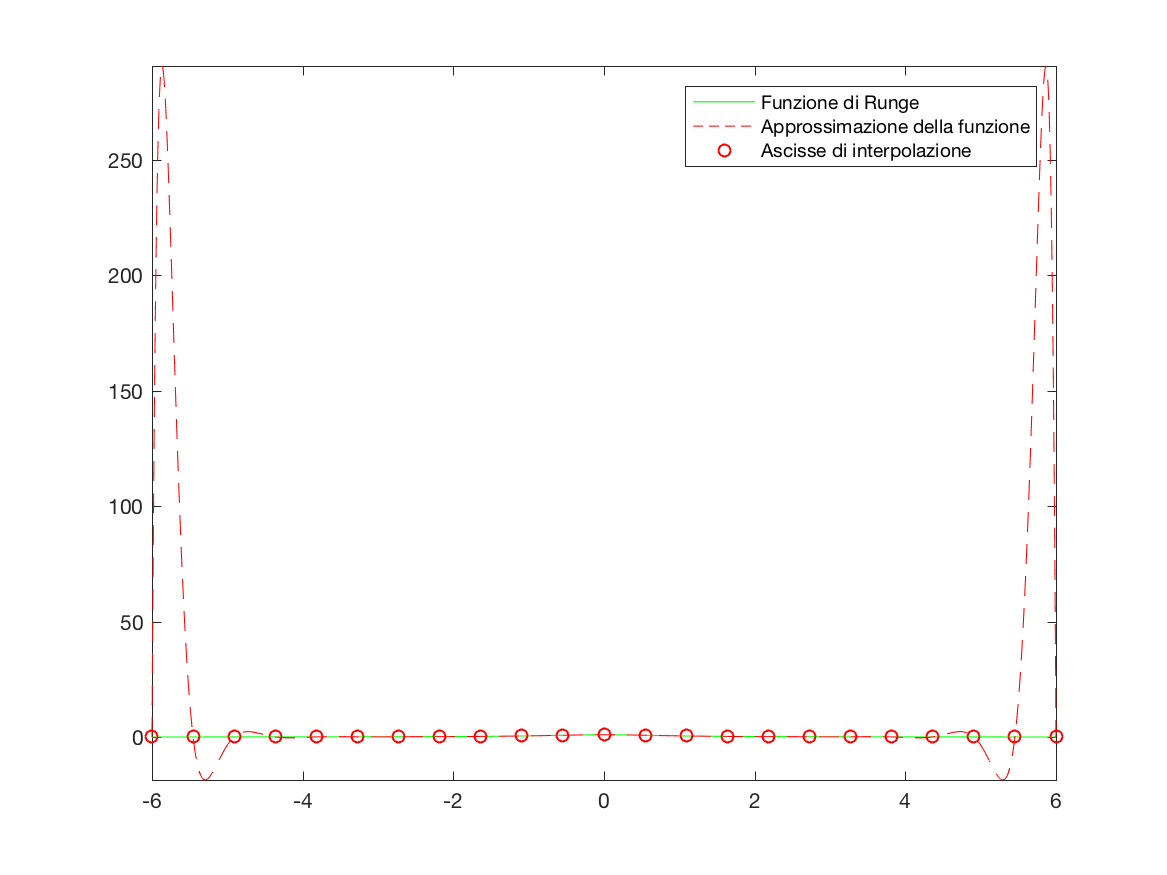
\includegraphics[scale=0.333]{Capitolo4/graficiEs9/es4_9_img22.png} \\
\end{tabular} \\
\begin{tabular}{cc}
\(n=28\) & \(n=34\) \\
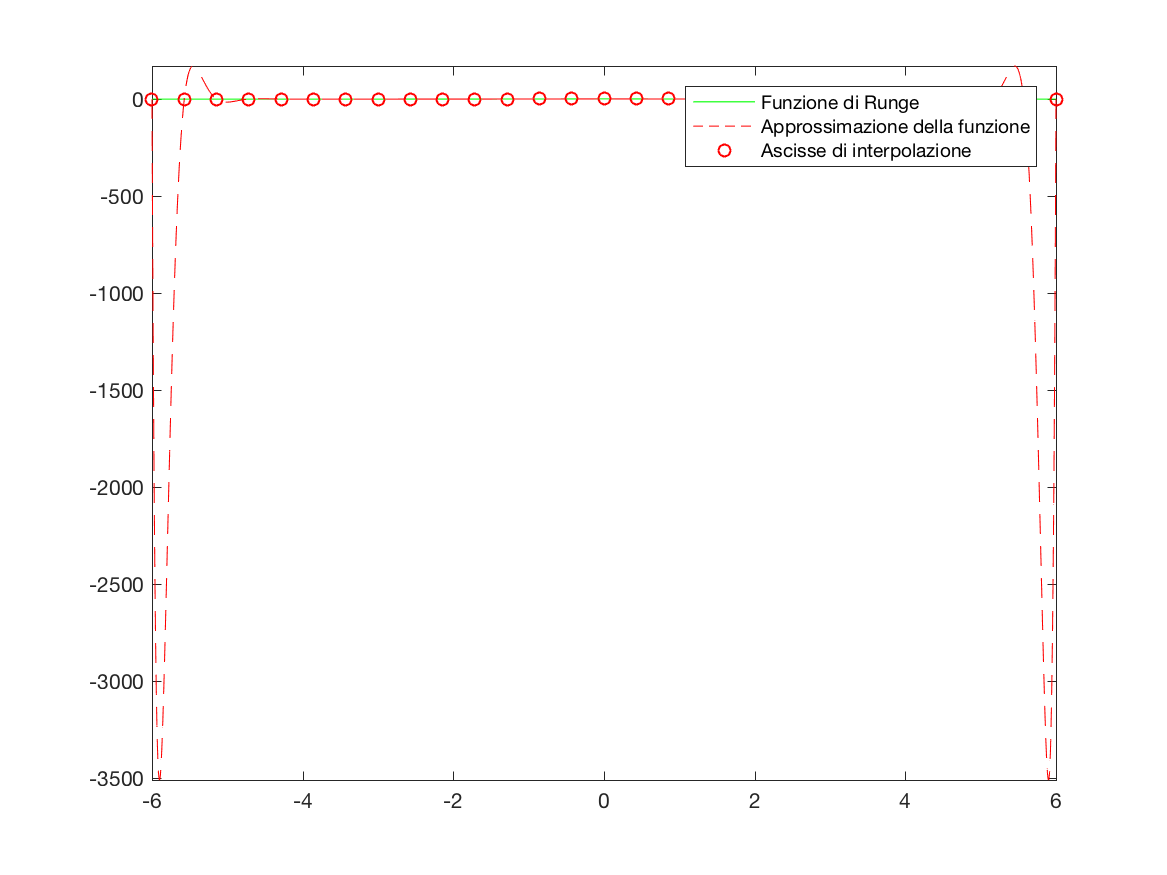
\includegraphics[scale=0.333]{Capitolo4/graficiEs9/es4_9_img28.png} &  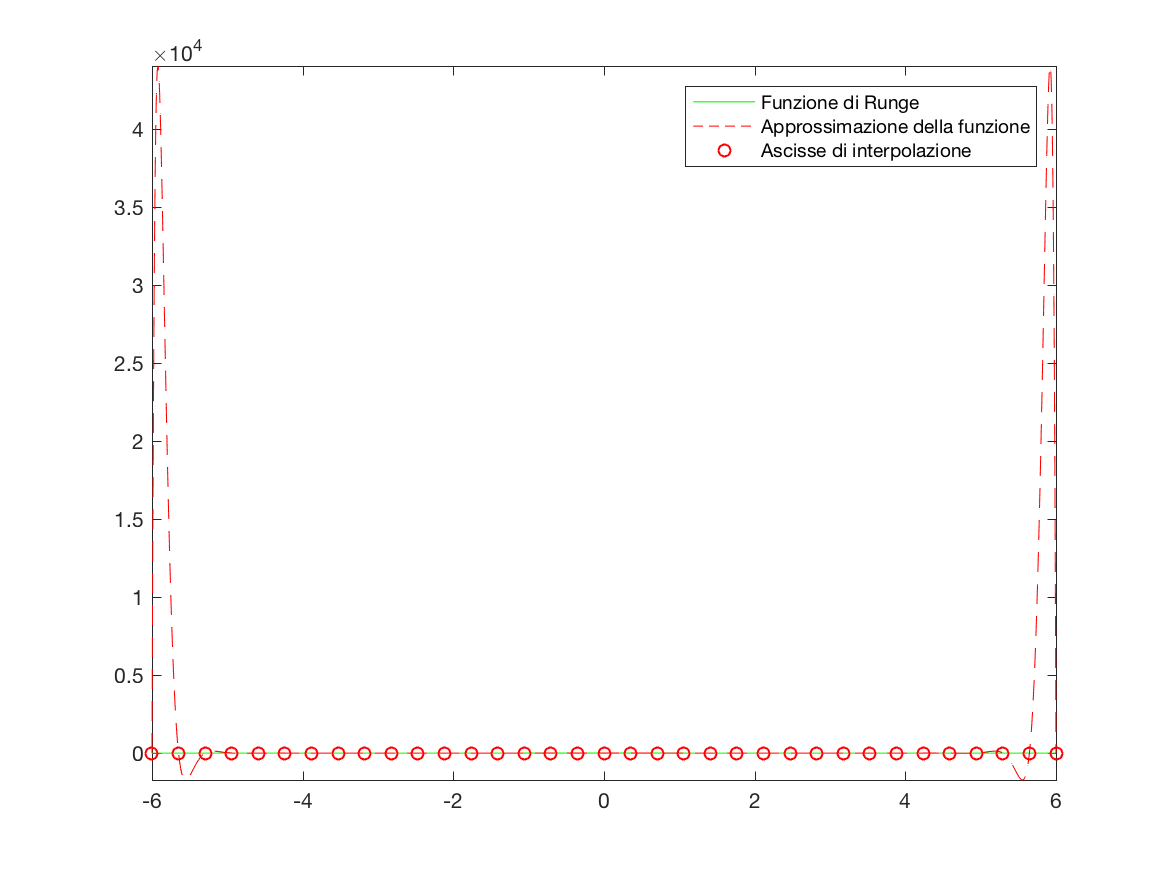
\includegraphics[scale=0.333]{Capitolo4/graficiEs9/es4_9_img34.png} \\
\(n=40\) &  \\
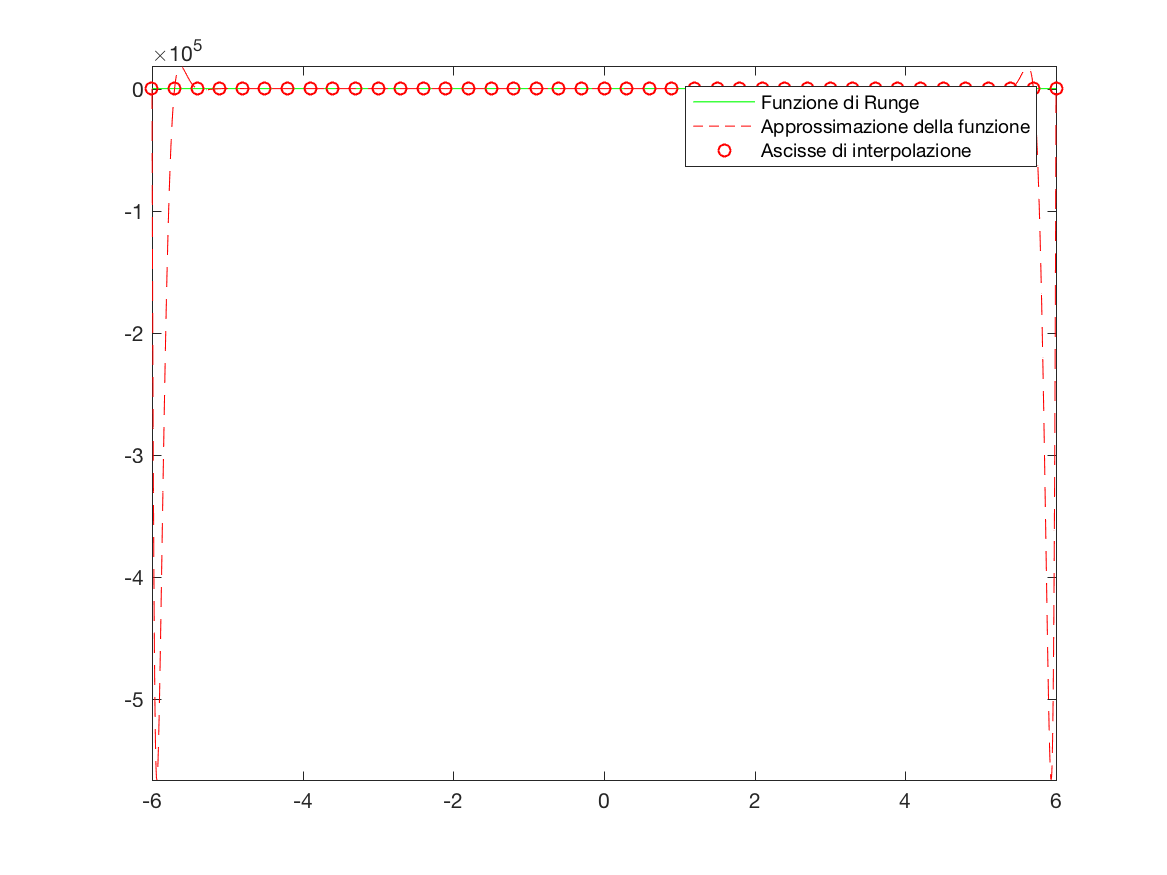
\includegraphics[scale=0.333]{Capitolo4/graficiEs9/es4_9_img40.png} &  \\
\end{tabular} \\
Di seguito riportiamo la tabella con le stime degli errori e della costante di Lebesgue in funzione del grado n:
\begin{center}
	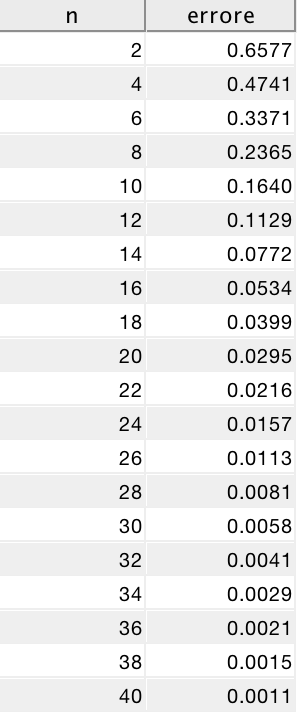
\includegraphics[scale=0.333]{Capitolo4/es4_9_tabella.png}
\end{center}
\bigskip
\textbf{Esercizio 4.10} \textit{Stimare, nel senso dei minimi quadrati, posizione, velocit� iniziale ed accelerazione relative ad un moto rettilineo uniformemente accelerato per cui sono note le seguenti misurazioni dele coppie (tempo, spazio):\\
\((1, 2.9) \quad (1, 3.1)\quad (2, 6.9) \quad (2, 7.1) \quad (3, 12.9) \quad (3, 13.1) \quad (4, 20.9) \quad (4, 21.1)\)\\\((5, 30.9) \quad (5, 31.1)\)}\\
\textbf{Soluzione: }Il problema posto consiste nel risolvere\\
\[
y = s(t) = x_{0} + v_{0}t + \frac{1}{2}at^{2}, \qquad \text{con } a, x_{0} \text{ e } v_{0} \text{ costanti}
\]
La stima, nel senso dei minimi quadrati, equivale alla risoluzione del sistema lineare sovradeterminato Ax=b:
\[
\begin{pmatrix}1 & 1 & 1 \\ 1 & 1 & 1 \\ 1 & 2 & 4 \\ 1 & 2 & 4 \\ 1 & 3 & 9 \\ 1 & 3 & 9 \\ 1 & 4 & 16 \\ 1 & 4 & 16 \\ 1 & 5 & 25 \\ 1 & 5 & 25 \end{pmatrix} \begin{pmatrix}x \\ v \\  a/2\end{pmatrix} = \begin{pmatrix} 2.9\\3.1\\6.9\\7.1\\12.9\\13.1\\20.9\\21.1\\30.9\\31.1 \end{pmatrix}
\]
Il problema � ben posto ed esiste un'unica soluzione in quanot abbiamo misurazioni in $n+1$ ascisse.\\
La matrice A � una matrice di Vandermonde con rango massimo 3. \\
\'E possibile calcolare una soluzione per il sistema dato utilizzando le function per la risoluzione e fattorizzazione dei sistemi QR sviluppati negli eserci precedenti:
\[
\begin{pmatrix}x\\v\\a/2 \end{pmatrix} = \begin{pmatrix}1\\1\\0.99999\end{pmatrix}
\]
\end{flushleft}
